\documentclass[aspectratio=169,11pt]{beamer}

% Shared style (ib-tutorials.sty at the repo root).
\makeatletter\def\input@path{{./}{../}}\makeatother
\usepackage{ib-tutorials}

\usepackage[utf8]{inputenc}
\usepackage{amsmath,amssymb}
\usepackage{booktabs}
\usepackage{array}
\newcolumntype{L}[1]{>{\raggedright\arraybackslash}p{#1}}
\usepackage{graphicx}
\graphicspath{{../pictures/appendices/}{pictures/appendices/}}
\usepackage{xcolor}
\usepackage{listings}
\usepackage{tikz}
\usetikzlibrary{arrows.meta,positioning,shapes.geometric,fit,calc}
\usepackage{hyperref}

\newcommand{\sourcecredit}[1]{\vfill\begin{flushright}\tiny\textcolor{DarkGray}{#1}\end{flushright}}

\lstset{
  basicstyle=\ttfamily\scriptsize\color{BlackGray},
  keywordstyle=\color{NavyBlue}\bfseries,
  commentstyle=\color{DarkGray}\itshape,
  stringstyle=\color{OliveGreen},
  showstringspaces=false,
  columns=fullflexible,
  keepspaces=true,
  breaklines=true,
  breakindent=1em,
  frame=single,
  framerule=0.4pt,
  rulecolor=\color{LightGray},
  backgroundcolor=\color{LightGray!30},
  xleftmargin=0.25em,
  xrightmargin=0.25em
}
\lstdefinestyle{shell}{morecomment=[l]{\#}}
\lstdefinestyle{python}{language=Python,morecomment=[l]{\#}}
\lstdefinestyle{matlab}{language=Matlab,morecomment=[l]{\%}}

\title[Appendix A: helper codes]{Appendix A: MATLAB and Python helper codes}
\subtitle{Every maintained MATLAB script of the series beside its Python version: the course exercises, the readers, the structure generators; how to run them, how they were checked against each other, and what to watch for when translating}
\author[Miller]{Laura A. Miller}
\institute[UArizona]{Department of Mathematics, University of Arizona}
\date{Using IB Software \textbullet\ Appendix A}

\begin{document}

% 1
\begin{frame}[plain]
\maketutorialtitlepanel{%
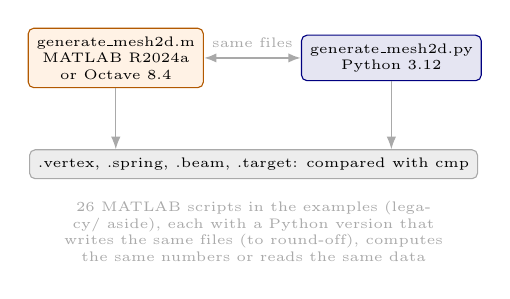
\begin{tikzpicture}[every node/.style={font=\tiny}, box/.style={draw, rounded corners=2pt, align=center, inner sep=3pt, minimum width=2.3cm}, arr/.style={{Latex[length=1.6mm]}-{Latex[length=1.6mm]},thick,DarkGray}]
  \node[box,draw=orange!70!black,fill=orange!10,minimum width=2.2cm] (m) at (0,0) {\code{generate\_mesh2d.m}\\MATLAB R2024a\\or Octave 8.4};
  \node[box,draw=NavyBlue,fill=NavyBlue!10,minimum width=2.2cm] (p) at (3.5,0) {\code{generate\_mesh2d.py}\\Python 3.12};
  \draw[arr] (m) -- node[above]{same files} (p);
  \node[box,draw=DarkGray,fill=LightGray!40,minimum width=5.5cm] (f) at (1.75,-1.35) {\code{.vertex}, \code{.spring}, \code{.beam}, \code{.target}: compared with \code{cmp}};
  \draw[-{Latex[length=1.6mm]},DarkGray] (m.south) -- (f.north -| m.south);
  \draw[-{Latex[length=1.6mm]},DarkGray] (p.south) -- (f.north -| p.south);
  \node[text=DarkGray,align=center,text width=5.4cm] at (1.75,-2.2) {26 MATLAB scripts in the examples (\code{legacy/} aside), each with a Python version that writes the same files (to round-off), computes the same numbers or reads the same data};
\end{tikzpicture}}
\end{frame}

% 2
\begin{frame}{Learning goals}
\label{fr:goals}
By the end of this appendix you should be able to:
\begin{enumerate}
  \item find the Python version of any MATLAB script of the series, and the chapter that uses it;
  \item run the course's four small exercises in MATLAB, Octave or Python, and read what they show;
  \item check that two versions of a generator write the same structure files, and know which differences are round-off;
  \item translate a MATLAB script to Python without the usual slips (indices from 1 or 0, ranges, array shapes, plots on a cluster).
\end{enumerate}
\begin{punchbox}
\small Use whichever language you have for the 26 MATLAB scripts of the examples: each has a Python version, and the pairs were run against each other in Octave 8.4, MATLAB R2024a and Python 3.12 (Octave has no \code{h5read}, which \code{samrai\_dumps.m} needs). The other 40 Python scripts of the examples have no MATLAB version (slide \ref{fr:where2}).
\end{punchbox}
\end{frame}

% 3
\begin{frame}{Where the MATLAB scripts are (1/3): with their Python versions}
\label{fr:where}
\scriptsize
\renewcommand{\arraystretch}{1.0}
\begin{tabular}{@{}L{0.28\textwidth}L{0.33\textwidth}L{0.33\textwidth}@{}}
\toprule
folder & MATLAB & Python \\
\midrule
\code{examples/support/\allowbreak{}matlab-exercises} & \code{heat\_equation.m}, \code{stiff\_ode\_example.m}, \code{test\_IB2d\_IBAMR\_Geometry.m}, \code{read\_Vertex\_Points\_\allowbreak{}and\_Plot\_Them.m} & \code{heat\_equation.py}, \code{stiff\_ode\_example.py}, \code{test\_ib\_geometry.py}, \code{read\_vertex\_points\_\allowbreak{}and\_plot\_them.py} \\
\code{examples/analysis} & \code{read\_hier\_data.m}, \code{read\_input.m}, \code{leaf\_forces.m}, \code{samrai\_dumps.m}, \code{read\_vtk\_legacy.m}, \code{read\_exodus.m}, \code{read\_curve.m} & \code{hier\_data.py} (with \code{read\_input}), \code{leaf\_forces.py}, \code{samrai\_dumps.py}, \code{read\_vtk\_legacy.py}, \code{read\_exodus.py}, \code{read\_curve.py} \\
\code{examples/IB/*} & \code{generate\_mesh2d.m} (01, 03, 04, 06, 07, 09--12), \code{Channel\_Flow.m} (02), \code{generate\_mesh3d.m} (08) & \code{generate\_mesh2d.py}, \code{channel\_flow.py}, \code{generate\_mesh3d.py} \\
\code{examples/ConstraintIB/*} & \code{Cylinder2d.m} (01, 02), \code{eel2d\_straightswimmer.m} (03) & \code{generate\_cylinder2d.py}, \code{generate\_eel2d.py} \\
\code{examples/IBFE/\allowbreak{}01-tethered-plate/\allowbreak{}extras} & \code{Beam\_IBFE\_Mesh2D.m} & \code{beam\_ibfe\_mesh2d.py} \\
\bottomrule
\end{tabular}

\vspace{1mm}
\footnotesize 26 \code{.m} files in all, outside \code{examples/legacy}: 4 course exercises, 7 readers, 15 structure generators. The scripts with no MATLAB version, and the older \code{.m} files, are on the next two slides.
\sourcecredit{The folders' \code{README.md} files (October 2026).}
\end{frame}

% 3b
\begin{frame}{Where the MATLAB scripts are (2/3): the scripts with no MATLAB version}
\label{fr:where2}
\footnotesize
\begin{itemize}\setlength{\itemsep}{2pt}
  \item \al{Python only} (no MATLAB version in this repository):
  \begin{itemize}\setlength{\itemsep}{1pt}
    \item in \code{analysis}: VisIt's scripts (\code{visit\_3d.py}, chapter 27; \code{visit\_queries.py}, 29; \code{visit\_movie\_frames.py}, 30; \code{resample\_export.py}, 33), the movie tools (\code{make\_movie.py}, \code{movie\_clean.py}, chapter 30), \code{flow\_rate.py}, \code{hier\_data\_h5.py} and \code{piv\_to\_vtk.py} (chapter 33), \code{vtk\_for\_planktos.py} (chapter 35);
    \item IB/11's \code{make\_inputs.py}, IB/13's \code{vessel\_walls.py} and \code{make\_input.py}, IBFE/05's \code{fix\_orientation.py};
    \item \code{examples/Planktos} (chapters 34 and 35), and the IB2d folders' Python (chapters 4c--4f, 19 files): generators, drivers and update functions ported from IB2d's own MATLAB examples (their originals stay in IB2d), the stability lab's \code{sweep.py} and \code{analyze.py}, the muscle-model scripts and \code{svg\_to\_vertex.py}.
  \end{itemize}
\end{itemize}
\sourcecredit{The folders' \code{README.md} files and the scripts' headers (October 2026).}
\end{frame}

% 3c
\begin{frame}{Where the MATLAB scripts are (3/3): the course versions, and the originals}
\label{fr:where3}
\footnotesize
\begin{itemize}\setlength{\itemsep}{3pt}
  \item \al{The course versions:} \code{examples/legacy} keeps 19 more \code{.m} files, the structure generators of the UNC and University of Arizona course folders as they were (\code{generate\_mesh2d.m}, \code{generate\_mesh3d.m}, \code{Channel\_Flow.m}, \code{Beam\_IBFE\_Mesh2D.m}, and \code{generate\_mesh2d\_plate.m} of a 2020 plate example that is not part of the series). They have no Python versions; 17 of them have a maintained successor among the examples of slide \ref{fr:where} (the seven identical copies of \code{Beam\_IBFE\_Mesh2D.m} are kept once, in IBFE/01's \code{extras}), and the two generators of the 2020 example have none (chapter 36).
  \item \al{The originals of the course exercises} are in \code{originals/MATLAB codes/}: \code{heat\_equation.m}, \code{stiff\_ode\_example.m}, and \code{test\_IB\_Geometry\_and\_Springs/} with the two plotting scripts and the rubber band they were run on.
\end{itemize}
\sourcecredit{The folders' \code{README.md} files and the scripts' headers (October 2026); chapter 36 on \code{legacy/}.}
\end{frame}

% 4
\begin{frame}[fragile]{Running them: MATLAB, Octave or Python}
\label{fr:run}
\begin{lstlisting}[style=shell]
matlab -batch "heat_equation(19,100)"        # MATLAB, from the script's folder
octave-cli --eval "heat_equation(19,100)"    # Octave: the same call, no desktop
python3 heat_equation.py 19 100              # Python 3 with NumPy and Matplotlib
python3 heat_equation.py 19 100 --show       # ... and open the plot in a window
\end{lstlisting}
\footnotesize
\begin{itemize}\setlength{\itemsep}{1pt}
  \item Versions used for this series: MATLAB R2024a, Octave 8.4, Python 3.12 (NumPy, Matplotlib; the readers also h5py for SAMRAI's HDF5 files and netCDF4 for Exodus).
  \item The Python versions save their plots as PNG files, so they also run on a cluster without a display; \code{--show} opens a window as well.
  \item Octave runs every \code{.m} file of \code{analysis} (with its \code{netcdf} package for \code{read\_exodus.m}) except \code{samrai\_dumps.m}, which needs MATLAB's \code{h5read}; MATLAB R2024a runs it (slide \ref{fr:readers}).
  \item With a display, \code{octave-cli} still opens a plot window (fltk); without one it draws with gnuplot (a text plot and a warning) and \code{heat\_equation.m} still writes \code{Example4\_1.eps}; with neither a display nor gnuplot, \code{heat\_equation.m}, \code{stiff\_ode\_example.m} and \code{Channel\_Flow.m} stop at their first plot.
  \item The ConstraintIB generators had their \code{plot} lines commented out so that \code{octave-cli} runs them on any machine: with a display or gnuplot Octave would draw the plot (or print it as text) and carry on, as it does for \code{Channel\_Flow.m} and the exercises, but with neither, the first plot stops the script before the file is written.
\end{itemize}
\sourcecredit{\code{examples/support/matlab-exercises/README.md}; \code{examples/analysis/README.md}; chapter 0.2 (versions).}
\end{frame}

% 5
\begin{frame}{The heat equation, and the stability of an explicit scheme (1/2)}
\label{fr:heat}
\begin{columns}[T,onlytextwidth]
\column{0.5\textwidth}
\centering
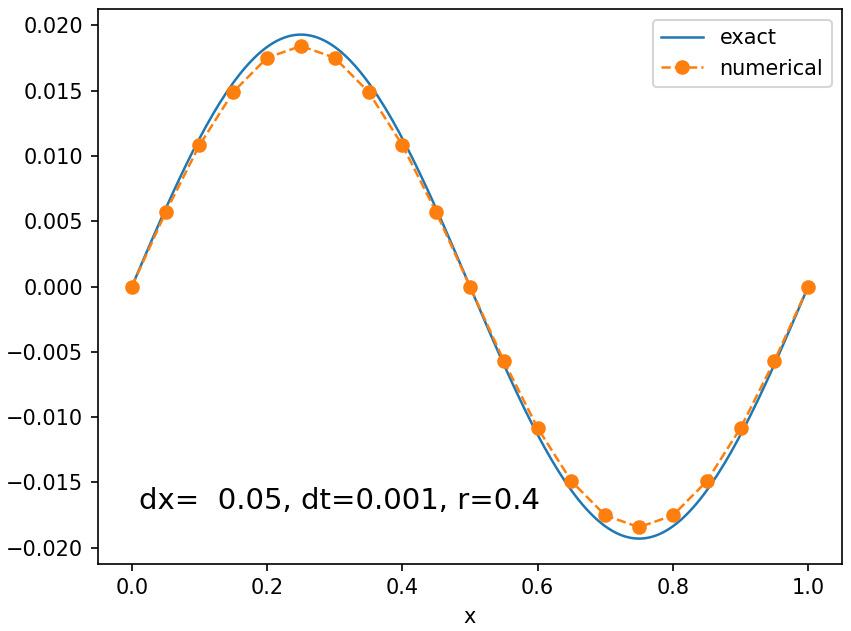
\includegraphics[width=\linewidth,height=0.42\textheight,keepaspectratio]{appA-heat-stable.png}

{\tiny\color{DarkGray}\code{heat\_equation.py 19 100}: $r = 0.4$, stable.\par}
\column{0.48\textwidth}
\centering
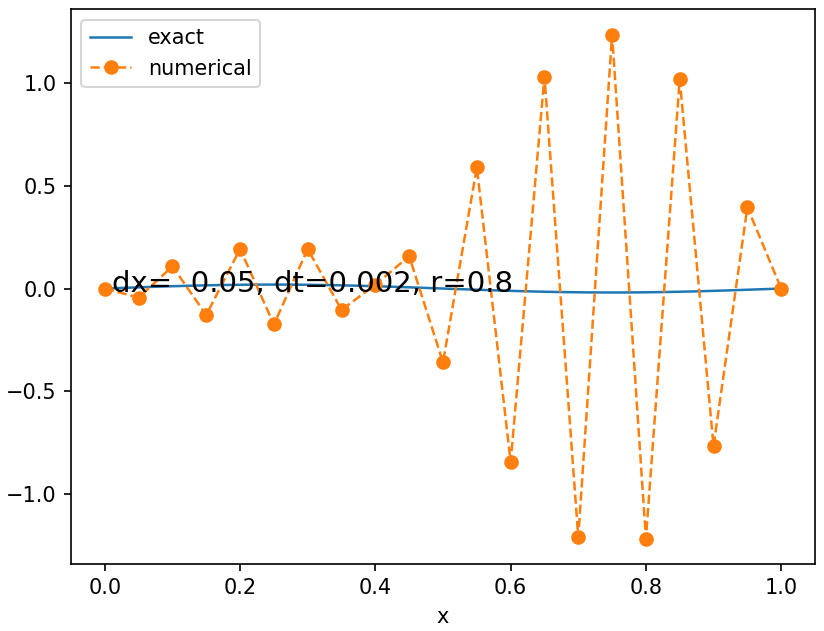
\includegraphics[width=\linewidth,height=0.42\textheight,keepaspectratio]{appA-heat-unstable.png}

{\tiny\color{DarkGray}\code{heat\_equation.py 19 50}: $r = 0.8$, unstable.\par}
\end{columns}
\footnotesize
\begin{itemize}\setlength{\itemsep}{1pt}
  \item $u_t = u_{xx}$ on $0 < x < 1$, $u(0) = u(1) = 0$, $u(x,0) = \sin 2\pi x$, to $t = 0.1$, against the exact $e^{-4\pi^2 t}\sin 2\pi x$. \code{N} interior points ($\Delta x = 1/(N+1)$), \code{T} steps ($\Delta t = 0.1/T$).
  \item Stable only for $r = \Delta t/\Delta x^2 \le 1/2$: largest error $8.7\times10^{-4}$ at $r = 0.4$ everywhere; at $r = 0.8$, $1.25$ in Python on Windows (the picture), $1.50$ in Python on Linux, $1.30$ in MATLAB R2024a and $5.3$ in Octave 8.4, while the solution itself is $0.019$.
\end{itemize}
\sourcecredit{\code{examples/support/matlab-exercises/heat\_equation.py} (run for this appendix); chapters 5 and 4d use the same scheme as the model of an explicit time-step limit: IBAMR and IB2d treat the viscous term implicitly to avoid this one, and it is the explicit spring force whose limit they meet (chapter 8a).}
\end{frame}

% 5b
\begin{frame}{The heat equation, and the stability of an explicit scheme (2/2): round-off grows}
\label{fr:heat2}
\footnotesize
\begin{itemize}\setlength{\itemsep}{3pt}
  \item The size differs because the growth starts from round-off at any $r > 1/2$: the grid's $\sin 2\pi x$ is a mode the scheme damps ($\times0.92$ per step at $r = 0.8$; with 60-digit arithmetic the error stays $2.3\times10^{-3}$), and the zigzag mode, seeded by rounding errors near $10^{-16}$, grows $\times2.18$ per step, $10^{17}$ in 50 steps. Just above $1/2$ ($r = 0.57$, \code{19 70}) it grows $\times1.27$ per step, $2\times10^{7}$ in 70 steps, and is still too small to see.
\end{itemize}
\sourcecredit{The runs for this appendix: Python 3.12 on Windows and on Linux, MATLAB R2024a, Octave 8.4, and a 60-digit run (mpmath) of the same scheme.}
\end{frame}

% 6
\begin{frame}{A stiff equation and Euler's method}
\label{fr:stiff}
\begin{columns}[T,onlytextwidth]
\column{0.46\textwidth}
\centering
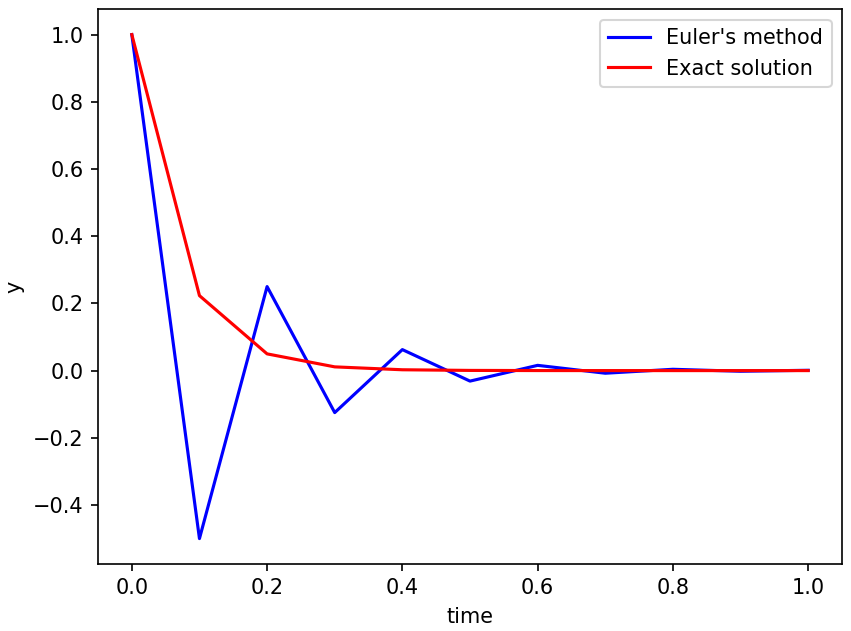
\includegraphics[width=\linewidth,height=0.55\textheight,keepaspectratio]{appA-stiff-ode.png}

{\tiny\color{DarkGray}\code{stiff\_ode\_example.py 0.1 1}: stable, but the sign flips every step.\par}
\column{0.52\textwidth}
\footnotesize
\begin{itemize}\setlength{\itemsep}{2pt}
  \item $y' = -15y$, $y(0) = 1$, exact $e^{-15t}$. Each Euler step multiplies $y$ by $1 - 15\Delta t$.
  \item $\Delta t < 1/15$: smooth decay (\code{0.05}); $1/15 < \Delta t < 2/15$: the sign alternates while the size decays (\code{0.1}, the picture); $\Delta t > 2/15 = 0.133$: it grows (\code{0.15}).
  \item The point for the IB method: stiff springs make the equations of motion stiff, and an explicit step must shrink with the stiffness: here, with no inertia, $\Delta t < 2/15$ ($\propto 1/\lambda$ for $y' = -\lambda y$); for the springs of chapter 8a's rule, which move fluid mass, $\Delta t \propto 1/\sqrt{k}$ (four times the stiffness, half the step).
  \item Changes from the course version: \code{zeros(N)} made $N\times N$ matrices (the plot drew $N$ curves), and the time grid stopped one step short of \code{tfinal}.
\end{itemize}
\end{columns}
\sourcecredit{\code{examples/support/matlab-exercises/stiff\_ode\_example.py} and its README; chapters 4d, 5, 8a and 16.}
\end{frame}

% 7
\begin{frame}{Checking a structure before running it}
\label{fr:geom}
\begin{columns}[T,onlytextwidth]
\column{0.42\textwidth}
\centering
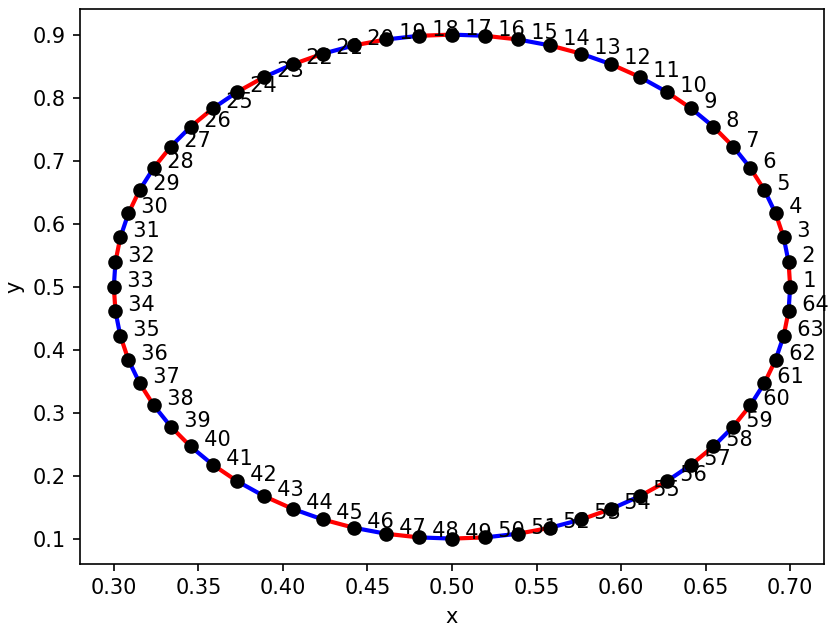
\includegraphics[width=\linewidth,height=0.6\textheight,keepaspectratio]{appA-rubberband-springs.png}

{\tiny\color{DarkGray}\code{test\_ib\_geometry.py rubberband}: 64 points with their numbers, the springs in alternating colours.\par}
\column{0.56\textwidth}
\scriptsize
\begin{itemize}\setlength{\itemsep}{2pt}
  \item \code{test\_ib\_geometry.py NAME [--ibamr]} (Python) / \code{test\_IB2d\_IBAMR\_Geometry.m} (MATLAB: the file names and \code{flag\_IBAMR = 0} or \code{1} are set at the top of the script): plots \code{NAME.vertex} with the point numbers, then the \code{NAME.spring} connections, so that a missing or crossed spring shows before the run does.
  \item IB2d numbers points from 1 (MATLAB) and IBAMR from 0 (C++): \code{--ibamr} labels from 0 and reads the springs that way. pyIB2d's files are 0-based too (chapter 4c).
  \item \code{read\_Vertex\_Points\_and\_Plot\_Them.m} / \code{read\_vertex\_points\_and\_plot\_them.py NAME}: the points alone.
  \item The 64-point IB2d rubber band in the folder is what they were run on: ``64 points, 64 springs'' in Python 3.12, MATLAB R2024a and Octave 8.4. Octave needed a fix (October 2026): its \code{textscan} does not end a row at the one-number count line, so the course versions misread the files there; both now read the count with \code{fgetl}.
\end{itemize}
\end{columns}
\sourcecredit{\code{examples/support/matlab-exercises} (run for this appendix); chapters 4a, 6 and 9a on structure files.}
\end{frame}

% 8
\begin{frame}{The structure generators (1/3): the examples of chapters 3--9}
\label{fr:gen1}
\scriptsize
\renewcommand{\arraystretch}{1.0}
\begin{tabular}{@{}L{0.18\textwidth}L{0.27\textwidth}L{0.48\textwidth}@{}}
\toprule
example & MATLAB / Python & checked \\
\midrule
IB/01 rubber band & \code{generate\_mesh2d.m} / \code{.py} & \code{.spring} identical; the shipped \code{.vertex} is MATLAB's (R2024a reproduces it exactly), and against it a few dozen of the 1288 coordinates differ in the last digit, by at most $1.4\times10^{-17}$ (44 in Octave 8.4 and in Python 3.12 on Linux, which agree with each other; 32 in Python on Windows): sine and cosine round differently in different math libraries \\
IB/02 pulsatile channel & \code{Channel\_Flow.m} / \code{channel\_flow.py} & the four files identical to the shipped ones \\
IB/03 tethered beam & \code{generate\_mesh2d.m} / \code{.py} & identical files (Octave 8.4, Python 3.12) \\
IB/04 moving cylinders & \code{generate\_mesh2d.m} / \code{.py} (new in 2026) & Python and Octave write exactly the shipped files; MATLAB R2024a differs in 9 of 594 coordinates, by $4\times10^{-19}$ m (its sine rounds one angle differently) \\
IB/06 growing springs, IB/07 moving plates & \code{generate\_mesh2d.m} / \code{.py} & identical files \\
\bottomrule
\end{tabular}
\sourcecredit{The examples' \code{README.md} files (October 2026).}
\end{frame}

% 9
\begin{frame}{The structure generators (2/3): the examples of chapters 9b, 10, 12 and 13}
\label{fr:gen2}
\scriptsize
\renewcommand{\arraystretch}{1.0}
\begin{tabular}{@{}L{0.2\textwidth}L{0.3\textwidth}L{0.43\textwidth}@{}}
\toprule
example & MATLAB / Python & checked \\
\midrule
IB/08 glycocalyx 3D & \code{generate\_mesh3d.m} / \code{.py} & \code{.target} identical; the shipped \code{.vertex} is MATLAB's (R2024a reproduces it); Octave 8.4 and Python 3.12 on Linux differ from it in the same 160 of the 40,800 coordinates, Python on Windows in 480, all in the last digit ($\le 1.7\times10^{-18}$ m) \\
IB/09, 10, 12 & \code{generate\_mesh2d.m} / \code{.py} & identical files (IB/12: the course's script with its beam loop fixed, which wrote a 170th beam, \code{169 170 171}, past the last point under a correct header of 169; the Python version new) \\
IB/11 heart-tube pump & \code{generate\_mesh2d.m} / \code{.py} & all 27 files identical between Octave 8.4 and Python 3.12 on one system; the shipped \code{heart\_race\_512.vertex} is Python-on-Windows output, and Octave or Python on Linux (101 of its 6,872 coordinates) and MATLAB R2024a (88) differ from it in the last digit ($\le 6\times10^{-17}$ m) \\
\bottomrule
\end{tabular}
\sourcecredit{The examples' \code{README.md} files; every generator run for this appendix in Octave 8.4, MATLAB R2024a and Python 3.12 (Windows and Linux).}
\end{frame}

% 9b
\begin{frame}{The structure generators (3/3): the examples of chapters 14 and 17, and the IBFE meshes}
\label{fr:gen3}
\scriptsize
\renewcommand{\arraystretch}{1.0}
\begin{tabular}{@{}L{0.2\textwidth}L{0.3\textwidth}L{0.43\textwidth}@{}}
\toprule
example & MATLAB / Python & checked \\
\midrule
ConstraintIB/01, 02 & \code{Cylinder2d.m} / \code{generate\_cylinder2d.py} & identical byte for byte in Octave 8.4 and Python 3.12, and equal to the file shipped upstream; MATLAB on Windows writes the same numbers with CRLF line endings (\code{fopen(..., 'wt')}): compare there with \code{diff --strip-trailing-cr} \\
ConstraintIB/03 & \code{eel2d\_straightswimmer.m} / \code{generate\_eel2d.py} & the same as 01 and 02: identical byte for byte, equal to upstream (CRLF from MATLAB on Windows) \\
IBFE/01 (extras) & \code{Beam\_IBFE\_Mesh2D.m} / \code{beam\_ibfe\_mesh2d.py} & the same Triangle \code{.poly} outline (not used by the example) \\
\bottomrule
\end{tabular}

\vspace{1mm}
\footnotesize The IBFE examples' meshes come from gmsh (IBFE/05, 10), Trelis (IBFE/08) or MATLAB's PDE Toolbox (IBFE/01, 06 and 12 share \code{IBFE\_Mesh2D\_128.mat}: the PDE Modeler, then a five-line \code{fprintf} script printed in IBFE/01's README and in chapter 17, with no \code{.m} file and no Python version); chapter 18 compares the routes. IB/13's walls come from \code{vessel\_walls.py} (Python only).
\sourcecredit{The examples' \code{README.md} files; \code{IBFE/01-tethered-plate/extras/README.md}; chapters 17 and 18.}
\end{frame}

% 10
\begin{frame}[fragile]{Checking that two versions agree (1/2): the recipe}
\label{fr:check}
\begin{lstlisting}[style=shell]
cp -r . /tmp/check && cd /tmp/check     # a copy: the mv lines empty the folder
shopt -s nullglob                       # skip the file types an example lacks
octave-cli generate_mesh2d.m && mkdir m && mv *.vertex *.spring *.beam *.target *.mass m/
python3 generate_mesh2d.py   && mkdir p && mv *.vertex *.spring *.beam *.target *.mass p/
for f in m/*; do cmp "$f" "p/$(basename $f)" && echo "same: $f"; done
\end{lstlisting}
\footnotesize
\begin{itemize}\setlength{\itemsep}{1pt}
  \item Same bytes is the best result, and most generators reach it: write numbers with the same format (\code{fprintf('\%1.16e')} and \code{'\%1.16e' \% x}) and compute them in the same order.
  \item Run from the example's folder (IB/01, 03, 04, 06, 07, 09--12). IB/02's, IB/08's, the ConstraintIB and IBFE/01's generators have other names (and IBFE/01's writes a \code{.poly} file): put their names in the two middle lines.
  \item Last-digit differences (about $10^{-16}$ relative, one or two units in the 17th significant digit: at most $1.4\times10^{-17}$ in IB/01, $4\times10^{-19}$ m in IB/04, $1.7\times10^{-18}$ m in IB/08, $6\times10^{-17}$ m in IB/11) are round-off: \code{sin} and \code{cos} differ between math libraries, between MATLAB and Octave (IB/01, 04, 08, 11) and between Python on Windows and on Linux (IB/01, 08, 11). Compare such files as numbers, \code{max(abs(a - b))}, not as text.
\end{itemize}
\sourcecredit{The recipe run on IB/01, 03 and 12 for this appendix; the READMEs' check notes.}
\end{frame}

% 10b
\begin{frame}{Checking that two versions agree (2/2): what the ports found}
\label{fr:check2}
\footnotesize
\begin{itemize}\setlength{\itemsep}{3pt}
  \item Anything larger than round-off is a bug in one of them.
  \item Porting also found bugs in the course scripts, some of which no comparison of outputs shows:
  \begin{itemize}\setlength{\itemsep}{1pt}
    \item a beam loop that ran one triple too far and wrote a 170th beam naming point 171 of a 171-point line (0--170) under a header of 169 (IB/12);
    \item \code{zeros(N)} where a vector was meant, so the plot drew $N$ curves, and a time grid one step short of \code{tfinal} (the stiff ODE);
    \item a comment that gave $\sin 3\pi x$ as the initial condition (the heat equation);
    \item a count line that Octave's \code{textscan} read together with the first point (the geometry checkers: in Octave one stopped, the other plotted each $y$ against the next point's $x$);
    \item in \code{samrai\_dumps.m}, written against the Python reader before MATLAB was at hand: \code{h5read} returns the variable names as strings since R2020a, and a variable named \code{cell} hid the function \code{cell}.
  \end{itemize}
  \item Only the beam line and the time grid change what the scripts write; the others change what they read, plot or say.
\end{itemize}
\sourcecredit{The READMEs' ``Changes from the course versions''; IB/12's README and the course's \code{examples/legacy/UNC-Examples/8-AddingMass-Spirder/spider2d\_256.beam} (its 170th line); the fixes of October 2026, run in Octave 8.4, MATLAB R2024a and Python 3.12.}
\end{frame}

% 11
\begin{frame}{The readers: the same data in MATLAB, Octave and Python}
\label{fr:readers}
\scriptsize
\renewcommand{\arraystretch}{1.0}
\begin{tabular}{@{}L{0.3\textwidth}L{0.4\textwidth}L{0.22\textwidth}@{}}
\toprule
MATLAB / Python & reads & chapter \\
\midrule
\code{read\_hier\_data.m} / \code{hier\_data.py} & the \code{X.*} and \code{F.*} files (PETSc ASCII) of \code{hier\_data\_IB2d} & 11 \\
\code{read\_input.m} / \code{hier\_data.read\_input} & a number from an input file, e.g.\ \code{DT} & 11 \\
\code{leaf\_forces.m} / \code{leaf\_forces.py} & IB/03's drag and lift: minus the sum of the forces on all 103 points of the leaf (the springs' and beams' forces cancel, so it is the pull of its two target points), and the ends' displacement & 11 \\
\code{samrai\_dumps.m} / \code{samrai\_dumps.py} & the fluid of a \code{visit\_dump.*} (SAMRAI HDF5): MATLAB's \code{h5read}; Python's h5py & 33 \\
\code{read\_vtk\_legacy.m} / \code{read\_vtk\_legacy.py} & VisIt's legacy ASCII VTK exports (resampled grids, meshes, points) and IB2d's \code{.vtk} output & 33 \\
\code{read\_exodus.m} / \code{read\_exodus.py} & IBFE's Exodus files (Octave's \code{netcdf}; netCDF4) & 33 \\
\code{read\_curve.m} / \code{read\_curve.py} & VisIt's \code{.curve} files, several curves per file kept apart & 29 \\
\bottomrule
\end{tabular}

\vspace{1mm}
\scriptsize Chapters 11 and 33 describe both versions of their readers (chapter 11: \code{read\_hier\_data}, \code{read\_input}, \code{leaf\_forces}; chapter 33: \code{samrai\_dumps}, \code{read\_vtk\_legacy}, \code{read\_exodus}), and chapter 29 runs both versions of \code{read\_curve} on its curve files (the pick through time: two curves in one file). The \code{.m} files ran in Octave 8.4 except \code{samrai\_dumps.m} (no \code{h5read} in Octave), which ran in MATLAB R2024a after two fixes (October 2026) and gives the same arrays as \code{samrai\_dumps.py}.
\sourcecredit{\code{examples/analysis/README.md}; chapters 11, 29 and 33.}
\end{frame}

% 12
\begin{frame}[fragile]{Translating MATLAB to Python (1/3): indices, ranges, shapes}
\label{fr:trans1}
\begin{columns}[T,onlytextwidth]
\column{0.41\textwidth}
\begin{lstlisting}[style=matlab,basicstyle=\ttfamily\fontsize{7.5}{9}\selectfont\color{BlackGray}]
x = 0:dx:1;            % includes 1
y = zeros(N,1);        % a column of N
for k = 1:N            % 1 ... N
    y(k) = sin(2*pi*x(k));
end
y(end)                 % the last one
fprintf(fid,'%d %1.16e\n', k-1, y(k));
\end{lstlisting}
\column{0.57\textwidth}
\begin{lstlisting}[style=python,basicstyle=\ttfamily\fontsize{7.5}{9}\selectfont\color{BlackGray}]
x = np.arange(N + 1) * dx  # 0 ... 1: count, don't step
y = np.zeros(N)            # zeros(N) in MATLAB is N x N
for k in range(N):         # 0 ... N-1
    y[k] = np.sin(2*np.pi*x[k])
y[-1]                      # the last one
f.write('%d %1.16e\n' % (k, y[k]))
\end{lstlisting}
\end{columns}
\footnotesize
\begin{itemize}\setlength{\itemsep}{1pt}
  \item \code{a:d:b} includes \code{b} when it lands on it (\code{0:0.1:0.3} has 4 points, the last 0.3); \code{np.arange(a, b, d)} is meant to stop before \code{b}, but with a float step round-off can add a point or lose one: \code{np.arange(1, 1.3, 0.1)} ends at 1.3. Build the grid from an integer count, \code{np.linspace(a, b, n)} or \code{a + d*np.arange(n)}.
  \item MATLAB indexes from 1, Python and IBAMR's structure files from 0 (IB2d's MATLAB files from 1, pyIB2d's from 0): shift the index when it is written into a file, not the loop.
\end{itemize}
\sourcecredit{The ports of this series (the support exercises, the generators, chapter 4c's IB2d ports).}
\end{frame}

% 13
\begin{frame}{Translating MATLAB to Python (2/3): arrays, numbers, files}
\label{fr:trans2}
\footnotesize
\begin{itemize}\setlength{\itemsep}{2pt}
  \item \al{Arrays:} \code{A*B} is a matrix product in MATLAB and element-wise in NumPy (\code{A @ B} for the product); \code{A'} is the conjugate transpose (\code{A.T} for real arrays). MATLAB's arrays are stored by columns, NumPy's by rows: when you reshape a flat list of values read from a file, say which order the file used (\code{order='F'} for column by column).
  \item \al{Integer division:} \code{floor(n/2)} in MATLAB, \code{n // 2} in Python; \code{/} on integers gives a float in Python 3.
  \item \al{Files:} \code{fprintf}'s conversions (\code{\%d}, \code{\%e}, \code{\%f}, \code{\%g}) mean the same in Python's \code{\%}-formatting, with two differences: \code{fprintf} repeats its format over every element of an array (\code{sprintf('\%d', [1 2 3])} is \code{123}; in Python, loop or use \code{np.savetxt}), and \code{\%d} of a number with a fraction, 2.5, prints \code{2.500000e+00} in MATLAB, \code{2.5} in Octave and \code{2} in Python. Write the same format and the files can be compared byte for byte (slide \ref{fr:check}).
\end{itemize}
\sourcecredit{The ports of this series; NumPy for MATLAB users, \url{https://numpy.org/doc/stable/user/numpy-for-matlab-users.html}.}
\end{frame}

% 13b
\begin{frame}{Translating MATLAB to Python (3/3): plots, functions and scripts}
\label{fr:trans3}
\footnotesize
\begin{itemize}\setlength{\itemsep}{2pt}
  \item \al{Plots:} save to a file (\code{plt.savefig}) and open a window only when asked, since a cluster job has no display: the exercises' Python versions save a PNG and open a window with \code{--show}; \code{channel\_flow.py} plots only with \code{--plot}. MATLAB and Octave can save a figure without showing it too (\code{figure('Visible','off')}, then \code{print} or \code{saveas}; \code{octave-cli} did so here without a display, through gnuplot, which Octave needs for any figure when there is no display). Of the MATLAB generators only IB/02's \code{Channel\_Flow.m} still opens a figure; the ConstraintIB ones have their \code{plot} lines commented out, so that \code{octave-cli} runs them even with neither a display nor gnuplot (slide \ref{fr:run}).
  \item \al{Functions and scripts:} a MATLAB function file becomes a Python function plus a \code{if \_\_name\_\_ == "\_\_main\_\_":} block that reads \code{sys.argv}, as \code{heat\_equation.py N T} does for \code{heat\_equation(N,T)}.
\end{itemize}
\sourcecredit{The ports of this series; the generators' and exercises' \code{README.md} files.}
\end{frame}

% 14
\begin{frame}{Exercises}
\label{fr:exercises}
\footnotesize
\begin{enumerate}\setlength{\itemsep}{2pt}
  \item Run \code{heat\_equation} with \code{19 100}, \code{19 70} and \code{19 50} in MATLAB or Octave and in Python; the \code{.m} file prints nothing, so add \code{max(abs(up - exp(-4*pi\textasciicircum{}2*t)*sin(2*pi*x)))} after its loop. Compare the largest errors, and explain why the languages (and one language on two systems) differ most in the unstable case.
  \item Find the largest $\Delta t$ for which \code{stiff\_ode\_example} decays without changing sign, and the largest for which it stays bounded; check them against $1/15$ and $2/15$.
  \item Run IB/03's two generators and compare their files with \code{cmp} (slide \ref{fr:check}); then IB/01's, and compare each \code{.vertex} with the shipped \code{rubber\_band\_512.vertex} (MATLAB's): measure the largest difference as numbers. On one Linux machine Octave and Python agree byte for byte; across systems they do not.
  \item Write the Python version of a small MATLAB script of your own; test it the same way.
  \item Read the same frame of \code{hier\_data\_IB2d/X.*} (from a run of IB/03 or another IB example: the repository ships no output) with \code{read\_hier\_data.m} and \code{hier\_data.py}, and check that the positions agree.
\end{enumerate}
\end{frame}

% 15
\begin{frame}{Summary and sources}
\label{fr:summary}
\footnotesize
\begin{itemize}\setlength{\itemsep}{2pt}
  \item 26 MATLAB scripts in the series' examples (\code{legacy/} aside), each with a Python version: 4 course exercises, 7 readers, 15 structure generators. Most generator pairs write identical files; the rest (IB/01, 04, 08, 11) differ by round-off in the last digit, which depends on the system, as their READMEs say. \code{samrai\_dumps.m} and the two geometry checkers were fixed in October 2026.
  \item MATLAB R2024a, Octave 8.4 or Python 3.12: use what you have. Python's versions save their plots and run on a cluster.
  \item When translating: count grid points instead of stepping, shift indices only when writing files, write the same number formats, and compare the outputs.
\end{itemize}
\vspace{1mm}
\footnotesize Sources: \code{examples/support/matlab-exercises}, \code{examples/analysis} and every example's \code{README.md} (October 2026); the course originals in \code{originals/MATLAB codes/}; NumPy's guide for MATLAB users.
\begin{punchbox}
\small The figures of this appendix were made by the Python versions, run for it.
\end{punchbox}
\end{frame}

\end{document}
